% Options for packages loaded elsewhere
\PassOptionsToPackage{unicode}{hyperref}
\PassOptionsToPackage{hyphens}{url}
%
\documentclass[
]{article}
\usepackage{amsmath,amssymb}
\usepackage{iftex}
\ifPDFTeX
  \usepackage[T1]{fontenc}
  \usepackage[utf8]{inputenc}
  \usepackage{textcomp} % provide euro and other symbols
\else % if luatex or xetex
  \usepackage{unicode-math} % this also loads fontspec
  \defaultfontfeatures{Scale=MatchLowercase}
  \defaultfontfeatures[\rmfamily]{Ligatures=TeX,Scale=1}
\fi
\usepackage{lmodern}
\ifPDFTeX\else
  % xetex/luatex font selection
\fi
% Use upquote if available, for straight quotes in verbatim environments
\IfFileExists{upquote.sty}{\usepackage{upquote}}{}
\IfFileExists{microtype.sty}{% use microtype if available
  \usepackage[]{microtype}
  \UseMicrotypeSet[protrusion]{basicmath} % disable protrusion for tt fonts
}{}
\makeatletter
\@ifundefined{KOMAClassName}{% if non-KOMA class
  \IfFileExists{parskip.sty}{%
    \usepackage{parskip}
  }{% else
    \setlength{\parindent}{0pt}
    \setlength{\parskip}{6pt plus 2pt minus 1pt}}
}{% if KOMA class
  \KOMAoptions{parskip=half}}
\makeatother
\usepackage{xcolor}
\usepackage[margin=1in]{geometry}
\usepackage{longtable,booktabs,array}
\usepackage{calc} % for calculating minipage widths
% Correct order of tables after \paragraph or \subparagraph
\usepackage{etoolbox}
\makeatletter
\patchcmd\longtable{\par}{\if@noskipsec\mbox{}\fi\par}{}{}
\makeatother
% Allow footnotes in longtable head/foot
\IfFileExists{footnotehyper.sty}{\usepackage{footnotehyper}}{\usepackage{footnote}}
\makesavenoteenv{longtable}
\usepackage{graphicx}
\makeatletter
\def\maxwidth{\ifdim\Gin@nat@width>\linewidth\linewidth\else\Gin@nat@width\fi}
\def\maxheight{\ifdim\Gin@nat@height>\textheight\textheight\else\Gin@nat@height\fi}
\makeatother
% Scale images if necessary, so that they will not overflow the page
% margins by default, and it is still possible to overwrite the defaults
% using explicit options in \includegraphics[width, height, ...]{}
\setkeys{Gin}{width=\maxwidth,height=\maxheight,keepaspectratio}
% Set default figure placement to htbp
\makeatletter
\def\fps@figure{htbp}
\makeatother
\setlength{\emergencystretch}{3em} % prevent overfull lines
\providecommand{\tightlist}{%
  \setlength{\itemsep}{0pt}\setlength{\parskip}{0pt}}
\setcounter{secnumdepth}{-\maxdimen} % remove section numbering
\ifLuaTeX
  \usepackage{selnolig}  % disable illegal ligatures
\fi
\usepackage[]{biblatex}
\addbibresource{ReferencesProject1.bib}
\IfFileExists{bookmark.sty}{\usepackage{bookmark}}{\usepackage{hyperref}}
\IfFileExists{xurl.sty}{\usepackage{xurl}}{} % add URL line breaks if available
\urlstyle{same}
\hypersetup{
  pdftitle={Assignment 1},
  hidelinks,
  pdfcreator={LaTeX via pandoc}}

\title{Assignment 1}
\author{}
\date{\vspace{-2.5em}}

\begin{document}
\maketitle

\section{Introduction}\label{introduction}

Portugal has been long celebrated for its wine production, from port
wine to \emph{vino verde} from the Minho province. To address growing
demand, the wine industry is interested in optimising its wine
production. As wine is a food product, most of its prized features are
taste and aroma, which are subjective measurements. Previous studies
have tried to categorise wine by quality through combining human taste
testers, physicochemical analysis and statistical methods in attempts to
introduce objectivity\footnote{\textcite{RN1}}. In this project, we are
most concerned with which \textbf{particular variables} are essential
for considering wine quality. By knowing which variables should be
prioritised, this can motivate further study on optimising the wine
according to essential attributes and enforce more efficient production.

Therefore, this report aims to address the following questions:

\begin{enumerate}
\def\labelenumi{\arabic{enumi}.}
\tightlist
\item
  Which variables play a significant role in ascertaining the quality of
  red and white wine?
\item
  Are there any trends between wine attributes and its perceived
  quality?
\item
  Are there any differences between mean acidity values of wine?
\item
  Are there any differences between mean sulfate/sulfur dioxide values
  of wine?
\end{enumerate}

The dataset employed in this study comprises data sourced from
laboratory tests, providing an intricate look into the chemical
composition of wines from Portugal's Minho region. It encompasses a
comprehensive range of variables, including fixed acidity, volatile
acidity, citric acid, residual sugar, chlorides, free sulfur dioxide,
total sulfur dioxide, density, pH levels, sulphates, alcohol content,
and a subjective quality rating on a scale of 0 to 10, where 10
represents the highest quality. Additionally, a color indicator, as a
dummy variable, distinguishes between red and white wines. - Data
checked for outliers - Total size is 6497 - To account for outliers but
also not to lose too much data, 5\% was chosen (325) entries as max
threshold to lose - Applied a IQR check. Normally, data less than Q1 -
IQR\emph{1.5 or more than Q3 + 1.5 }IQR is common procedure as it does
not assume normality - However, this lead to a large amount fo data
being lost, so stricter threshold of 2.5 was chosen instead.

\subsection{EDA - How does citric acid play a role in quality of
wines?}\label{eda---how-does-citric-acid-play-a-role-in-quality-of-wines}

\begin{itemize}
\tightlist
\item
  Citric acid plays a vital role in wine production
\item
  It helps add freshness to the wine, allowing more lively and enjoyable
  tasting experience, but too much makes it harsh, difficult to
  drink\footnote{\textcite{RN3}}
\item
  Therefore, we are interested in any trends between citric acid
  concentration and perceived wine quality
\item
  Question: Specific to wines of the minho region, what ranges of
  concentrations is related to wine quality?
  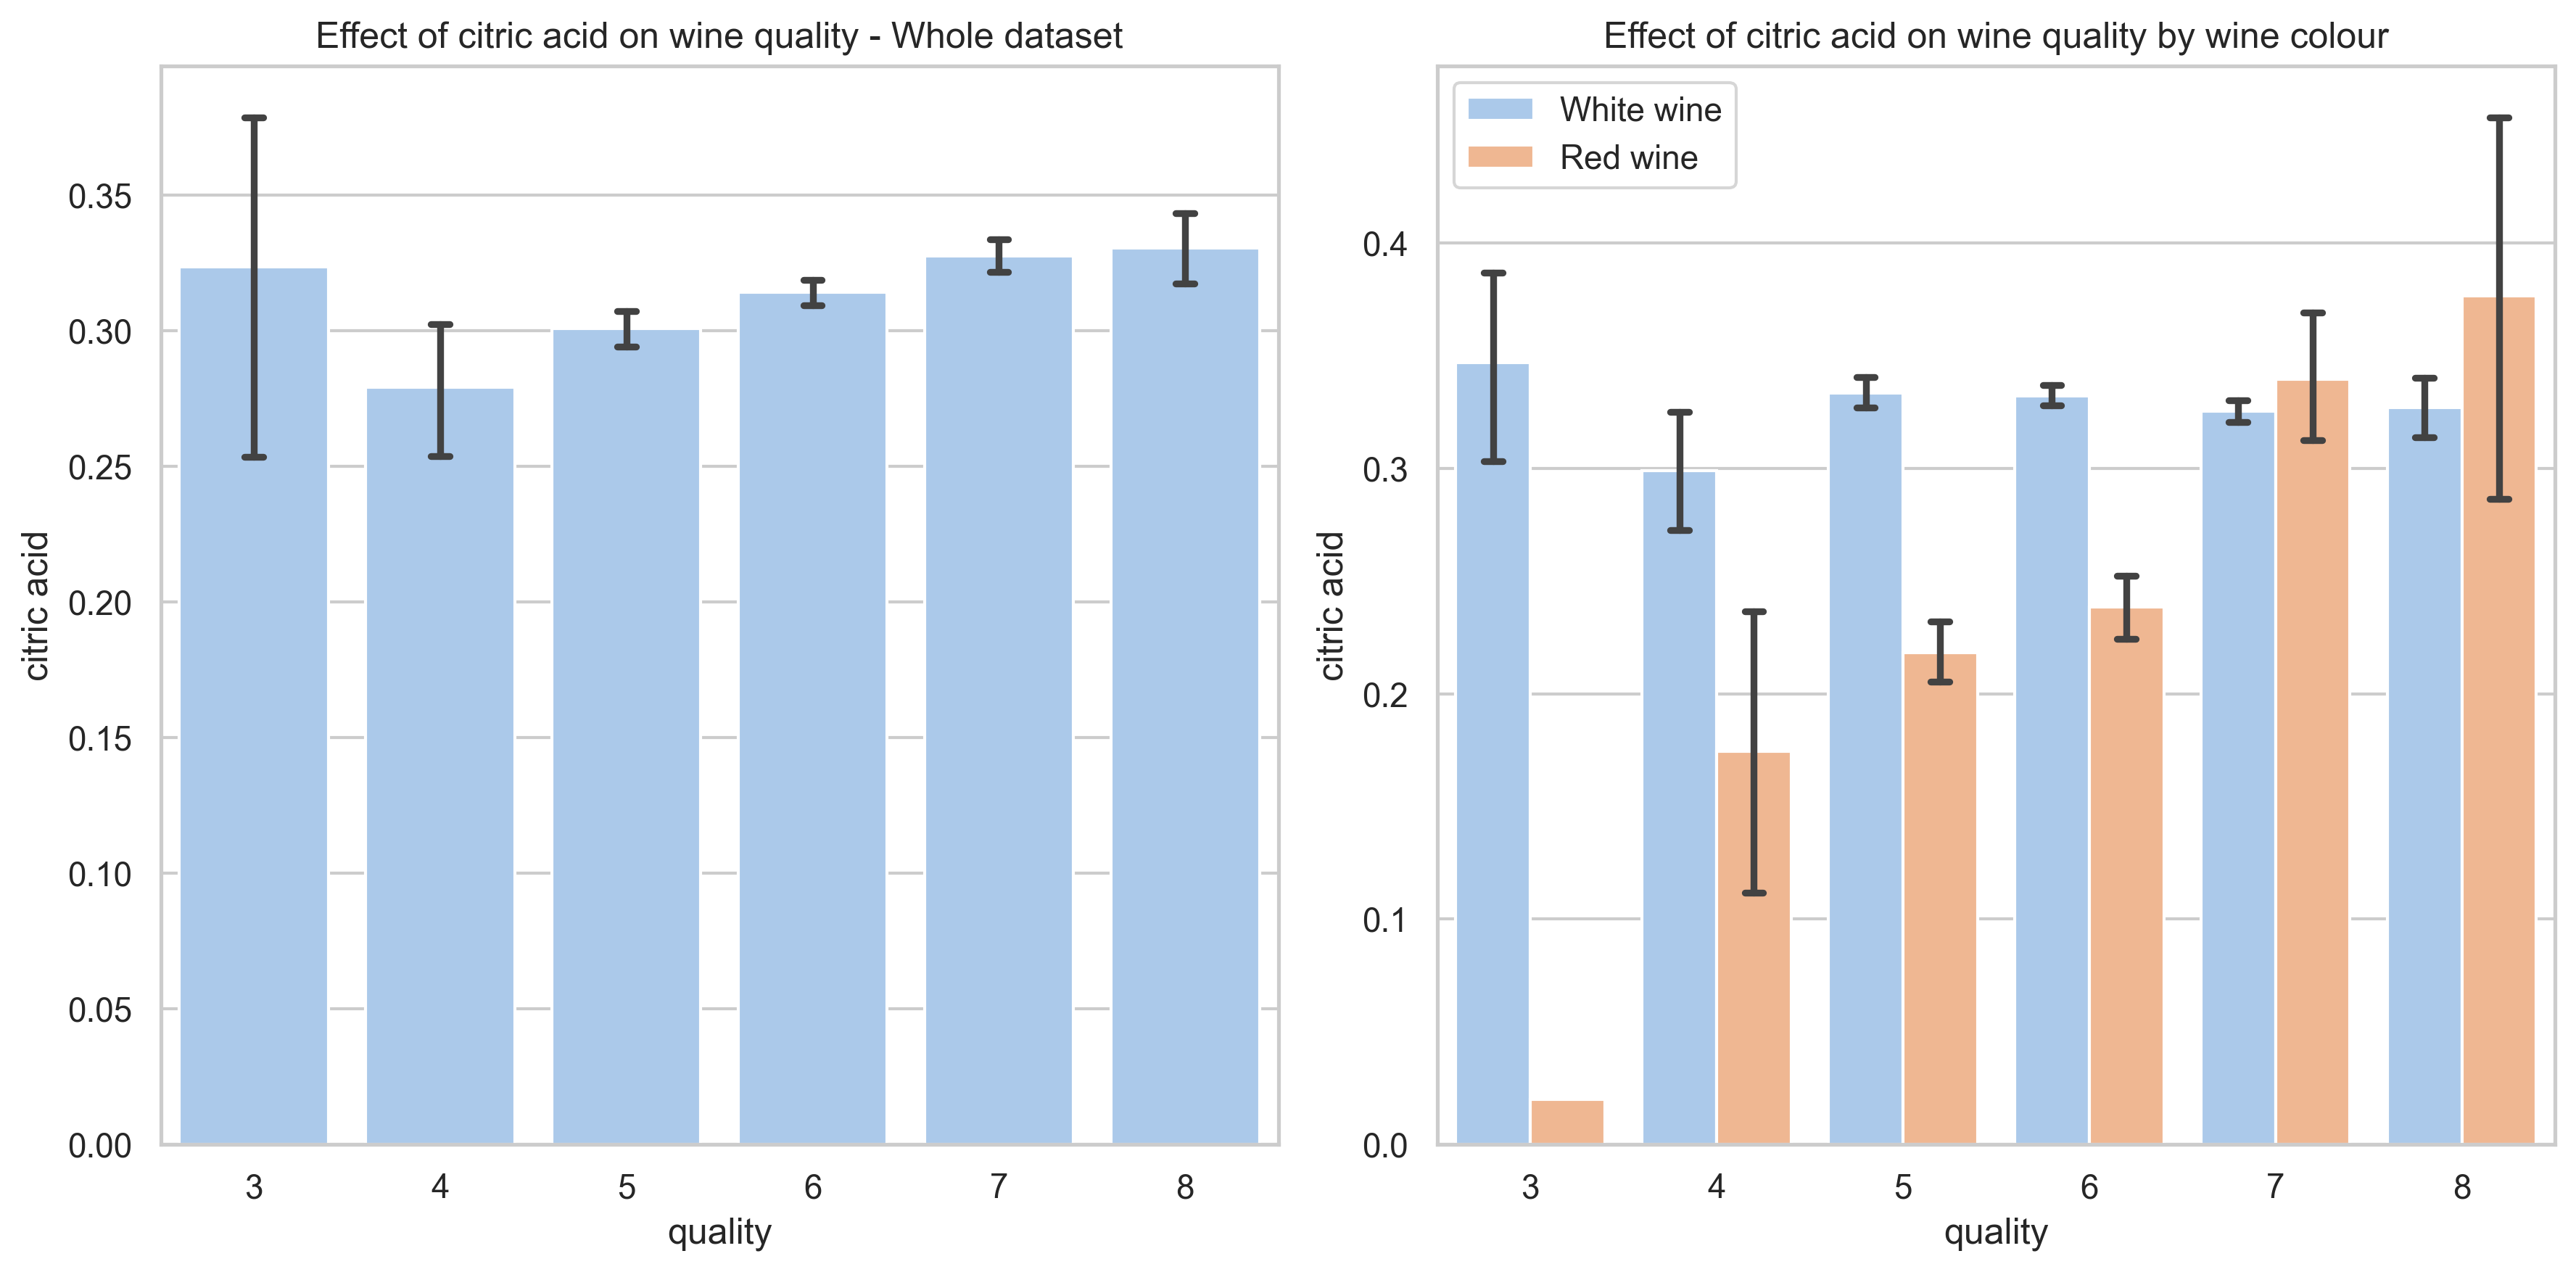
\includegraphics{whole_data_by_colour_citric_acid_vs_quality.png}
\item
  Across dataset:

  \begin{itemize}
  \tightlist
  \item
    High citric acid for low quality (but not certain due to low numbers
    in category 3 and large error bar)
  \item
    Steady increase from quality 4 to 8, but plateaus around 0.33
    g/dm\(^3\)
  \item
    Wines that are ``high quality'' tend to have citric acid
    concentrations between 0.30 g/dm\(^3\) and 0.35 g/dm\(^3\)
  \end{itemize}
\item
  Between wine groups:

  \begin{itemize}
  \tightlist
  \item
    In general, citric acid concentration over higher quality white wine
    seems to be fairly consistent, around 0.30 g/dm\(^3\) and 0.35
    g/dm\(^3\)
  \item
    Red wine much more drastic. Even after accounting for large error
    bars from smaller datapoints for red wine, there is a clear increase
    between higher quality wines have more citric acid
  \end{itemize}
\item
  Conclusion: It seems that higher quality red wines have more citric
  acid in them, but it is unclear whether red wine quality of 9 or
  higher will have more citric acid due to the large error bars. What is
  apparent is higher quality wines in general tend to have citric acid
  concentrations between 0.30 to 0.35 g/dm\(^3\). This disparity could
  be explained by how white wines tend to have more residual sugar than
  red wines, where adding some freshness is more necessary to balance
  out the additional sweetness.\footnote{\textcite{RN1}}
\end{itemize}

\subsection{PCA - Chemical differences between red and white
wines}\label{pca---chemical-differences-between-red-and-white-wines}


\includegraphics{Scree_plot.png} Looking at the scree plot, the elbow
appears around n = 3 components, so we will use this when proceeding
with our PCA model. When considering the key chemical differences
between red and white wines, we need to identify which features produce
large loadings for our model. These features will help maximumise the
langrange multiplier, producing the largest variance which is essential
in differentiating the chemical differences between red and white wines.

From the PC2 vs PC1 plot, we observe:

\begin{longtable}[]{@{}
  >{\raggedright\arraybackslash}p{(\columnwidth - 4\tabcolsep) * \real{0.3333}}
  >{\raggedright\arraybackslash}p{(\columnwidth - 4\tabcolsep) * \real{0.3333}}
  >{\raggedright\arraybackslash}p{(\columnwidth - 4\tabcolsep) * \real{0.3333}}@{}}
\toprule\noalign{}
\begin{minipage}[b]{\linewidth}\raggedright
\textbf{PC1 loading}
\end{minipage} & \begin{minipage}[b]{\linewidth}\raggedright
\textbf{PC2 loading}
\end{minipage} & \begin{minipage}[b]{\linewidth}\raggedright
\textbf{PC3 loading}
\end{minipage} \\
\midrule\noalign{}
\endhead
\bottomrule\noalign{}
\endlastfoot
Density is small and positive & Density is large and positive & Density
is close to zero \\
Fixed acidity is small and positive & Fixed acidity is small and
positive & Fixed acidity is large and positive \\
Chlorides is moderate and positive & Chlorides is small and positive &
Chlorides is close to zero \\
Volatile acidity is large and positive & Volatile acidity is small and
positive & Volatile acidity is small and negative \\
Colour is large and positive & Colour is small and positive & Colour is
close to zero \\
Sulphates is moderate and positive & Sulphates is close to zero &
Sulphates is small and positive \\
pH is moderate and positive & pH is small and negative & pH is large and
negative \\
Alcohol is close to zero & Alcohol is large and negative & Alcohol is
close to zero \\
Chlorides is moderate and positive & Chlorides is small and positive &
Chlorides is close to zero \\
Total sulfur dioxide is moderate and negative & Total sulfur dioxide is
small and positive & Total sulfur dioxide is small and negative \\
Free sulfur dioxide is small and negative & Free sulfur dioxide is
moderate and positive & Free sulfur dioxide is small and negative \\
Residual sugar is small and negative & Residual sugar is large and
positive & Residual sugar is small and negative \\
\end{longtable}

\begin{itemize}
\tightlist
\item
  So far, we have identified some differences for the wines considering
  citric acid concentration
\item
  However, what key attirbutes help differentiate red and white wines?
  This is necessary to ensuring we produce different wine types
  correctly
\item
  We can consider key chemical differences between the wines, as this
  are more objective measurements than human taste testers
\item
  Therefore, we will perform a princinple component analysis on our
  dataset, considering wine colour to be the key differentiator
\item
  A scree plot was produced fitting a PCA model to investigate the best
  number of components
\item
  From the plot, the elbow appears to be for 3 components, so this is
  what we will select
\item
  Following this, a plot of the loadings and fit was produced
  !(biplots\_combined){[}biplots\_combined\_no\_quality.png{]}
\item
  PC2 vs PC1:

  \begin{itemize}
  \tightlist
  \item
    Clear divide between white and red wines
  \item
    Higher loadings for PC1 gives higher loadings for PC2 for volatile
    acidity, fixed acidity, density, sulphates and chlorides
  \item
    The colour loading is in the second quadrant. This suggests that red
    wine (colour coded as 1) will tend to be more acidic, have more
    sulphates and chlorides
  \item
    This is further supported by pH. In chemistry, pH is a logarithmic
    measure. For example a pH of 2 is equivalent to 10\^{}-2
    concentration of proton ions. This means that lower pH values are
    more acidic, because acidity is defined as the concentration of
    protons in a solution. The fact that PC1 has a higher loading of pH
    but lower for PC2 is further evidence fo this.
  \item
    Furthermore, from the plot, we can see that residual sugar, free
    sulfur dioxide, total sulfure dixiode and citric acid have higher
    PC2 loadings but lower PC1 loadings. The fact the arrows are facing
    away from the colour arrow indicates they are indicators of white
    wines. In ohter words, white wines tend to have more residual sugar,
    citric acid, free sulfure dfioxide and total sulfur dixide. THis
    makes sense because sulfur dixoide is produced during the
    fermentation process. More sugar means more alcohol can be produced,
    hence more fermentation. This indicates that high sulfur dioxide and
    residual sugar levels are indicators of white wine.
  \item
    Alcohol loading is almost perfectly 0 for PC1 but large and negative
    for PC2. This suggests that alcohol concetnration has no association
    between red and white wines.
  \item
    Conclusion so far: More acidity is associated with red wines and
    more sugar and sulfur dioxide is associated with white wines
  \end{itemize}
\item
  PC3 vs PC2 allows further nuance in evaluiating the chemical
  differnces between red and white wines. This can be useful to consider
  secondary measures where taking intial measurements fo acidity and
  sulfure dixoide may give inconclusive results

  \begin{itemize}
  \tightlist
  \item
    Colour loading small and positive, so look at arrows close to it
  \item
    While for PC2 vs PC1 plot loadings showed no association between
    red/white wine and alcohol concentration, the loading for alcohol is
    present in the first quadrant. It is karge, negartive for PC2 but
    positive for PC3. As it is away from the colour variable, this
    indicates that white wines tend to have slightly more alcohol
    concentration than red wines.
  \item
    Fixed acidity is very strongly loaded for PC2 and PC3, indicating is
    a
  \item
    Most of the relationships are similar as seen inthe previous plot
  \item
    Conclusion: When used as a secondary measure, white wines tend to
    have higher alcohol concetntrations
  \end{itemize}
\item
  Overall conclusion: The main chemcial differences between red and
  white wines are concerned with acidity \#\# PCA analysis
\end{itemize}

\begin{enumerate}
\def\labelenumi{\arabic{enumi}.}
\tightlist
\item
  Plots of principle components
\item
  Comment on the main chemical differences between red and white wines
\item
  Including quality variable what features are likely to be present in
  wines of good quality? Is it different for red and white?
\end{enumerate}

\subsubsection{How to approach PCA}\label{how-to-approach-pca}

First, check the distributions of the data. You can do this using
cumulative variance or the plots from datacamp. Are there any werid
points?

If needed, transform the data. You can use make\_pipeline() to help you.

Display the variance and note the elbow of the plot. Which components
are necessary? What can be discarded?

Print out the PCAs as a table with an appropiate caption. Comment on a
few PCAs for contributions, relating back to some of the math, such as
the eigenvalues. Include a formula.

Your research question show address the following: ``What features are
most influential on a particular type of wine of high quality?'' You
should also consider the main chemical differences between red and white
wines (Use the PCA components for this)

\section{One page - Hotelling T square
test}\label{one-page---hotelling-t-square-test}

\begin{enumerate}
\def\labelenumi{\arabic{enumi}.}
\tightlist
\item
  Perform a Hotelling's \(T^2\) -test to test the hypothesis that the
  red and while wines have the same acidity means (the variables fixed
  acidity, volatile acidity and pH)
\item
  Select some variables and compute \(\mu_W\) of selected variables for
  white wine
\item
  Perform 1-sample \(T^2\) test to check whether corresponding means for
  red wine dataset are equal to \(\mu_W\)
\end{enumerate}

\subsection{Approaching the Hotelling T square
test}\label{approaching-the-hotelling-t-square-test}

\begin{enumerate}
\def\labelenumi{\arabic{enumi}.}
\tightlist
\item
  Give a sentence or two for motivation of test
\item
  Give a little math background
\item
  State the hypothesis clearly
\item
  Perform test
\item
  State the result with a confidence interval if applicable
\end{enumerate}

Your report should have: 1. A question stated clearly 2. Explaining the
statistical test used to address question 3. Give solution 4.
Potentially visualisation

Other notes: 1. You must give references 2. Try to keep it to 4 pages

\subsection{Things to keep in mind}\label{things-to-keep-in-mind}

\begin{itemize}
\tightlist
\item
  Citric acid and residual sugar levels are more important in white
  wine, where the equilibrium between the freshness and sweet taste is
  more appreciated
\item
  volatile acidity has a negative impact on wine taste, as it introduces
  bitterness (cite this)
\item
  Sulphastes might link to wine aroma
\item
  Additional research into impact of what affects wine tastes could
  prove useful.
\end{itemize}

\textcite{TODO} Sulphates formed from fermentation. More fermentation
=\textgreater{} more age =\textgreater{} more quality?

\printbibliography

\end{document}
